\begin{apendicesenv}
% \partapendices

\chapter{DESENHO TÉCNICO DO CHASSI}

Este apêndice apresenta o desenho técnico do chassi desenvolvido para o projeto, contendo dimensões e vistas estruturais.

\begin{itemize}
    \item Projeto: Chassi do protótipo
    \item Autor: Samara Sardinha Sousa
    \item Escala: 2:3
    \item Unidade: milímetros (mm)
\end{itemize}

\begin{figure}[H]
    \centering
    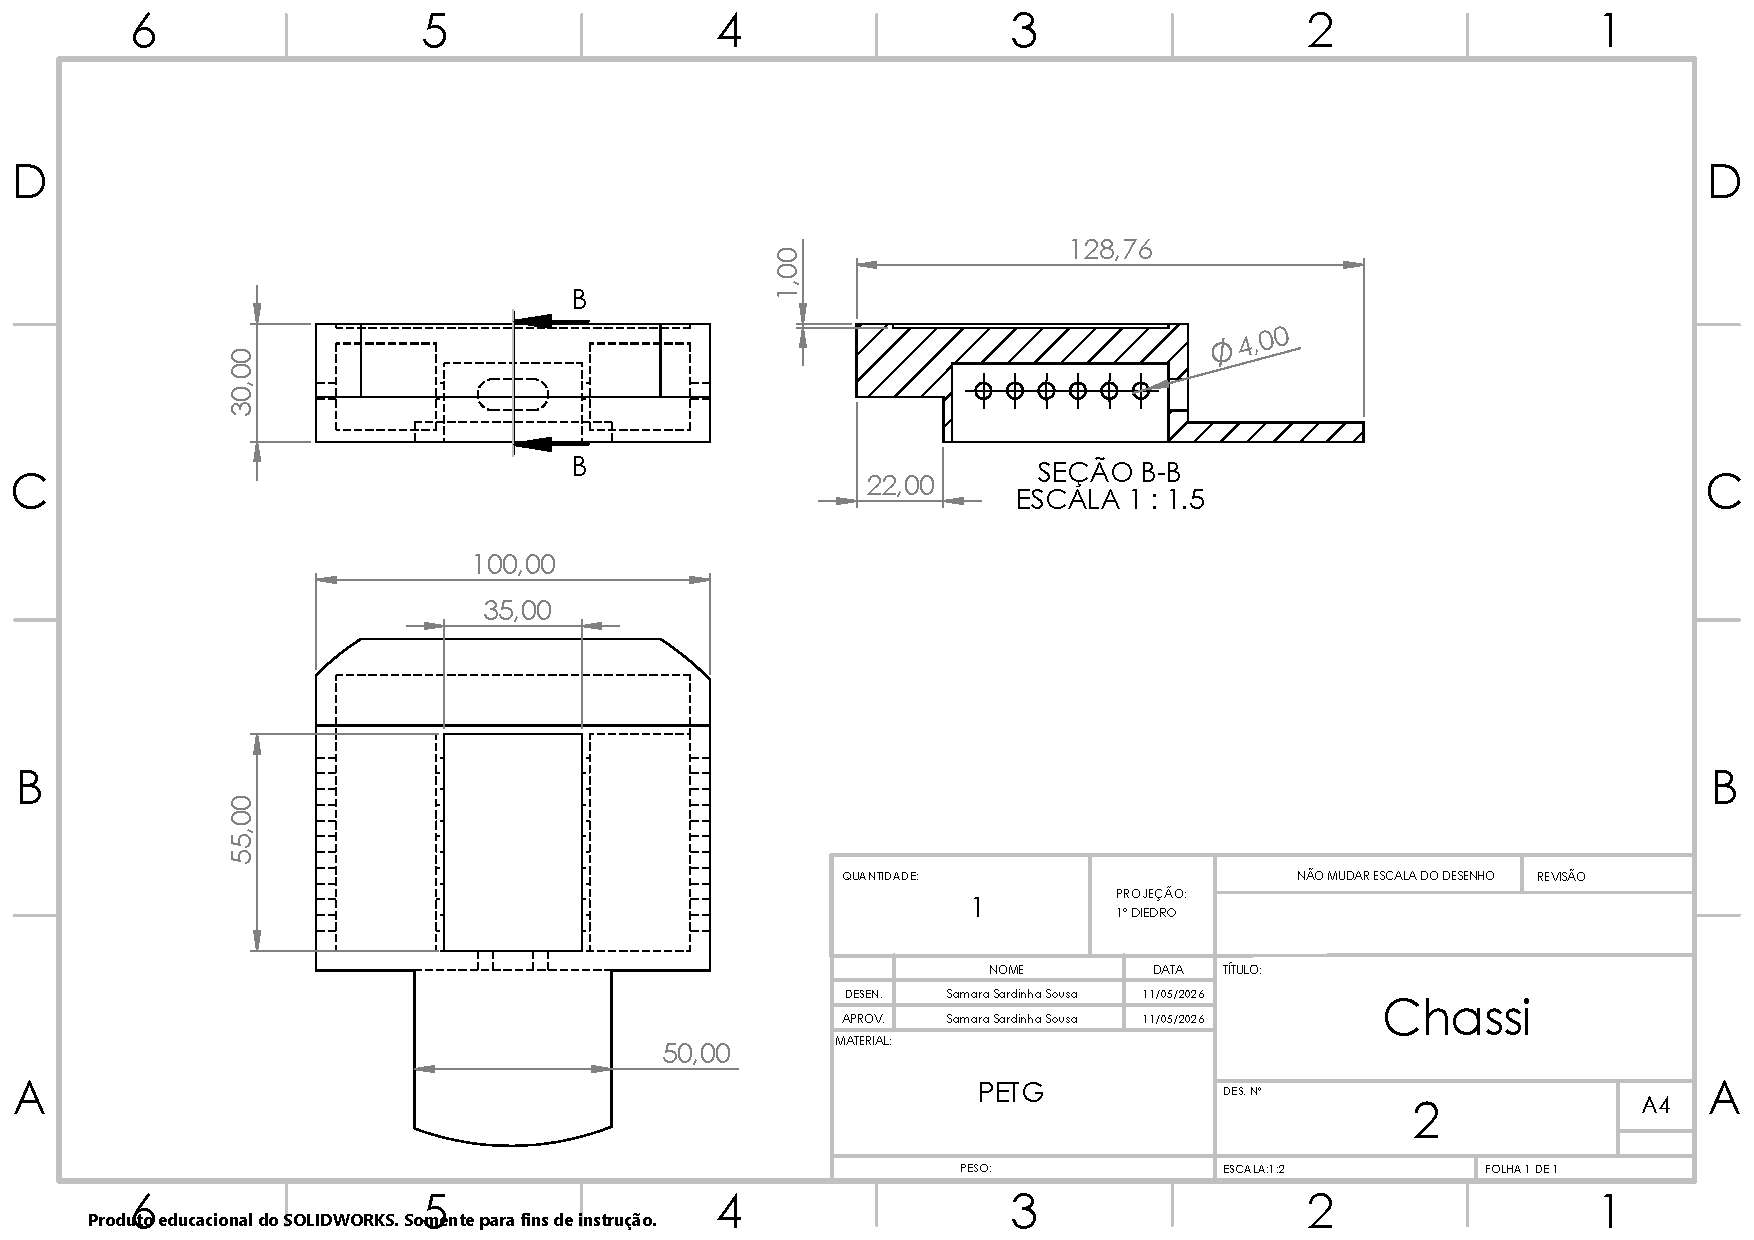
\includegraphics[width=1\linewidth]{figuras/chassi.pdf}
    \caption{Desenho técnico do chassi com vistas superior, lateral e frontal}
    \label{fig:chassi}
\end{figure}


\chapter{Segundo Apêndice}
\textcolor{red}{Apêndices e anexos são materiais complementares ao texto que só devem ser incluídos quando forem imprescindíveis à compreensão deste:}

\textcolor{red}{
\begin{itemize}
    \item Apêndices são textos elaborados pelo autor a fim de complementar sua argumentação.
    \item Anexos são os documentos não elaborados pelo autor, que servem de fundamentação, comprovação ou ilustração, como mapas, leis, estatutos etc.
\end{itemize}}

\textcolor{red}{\textbf{Texto do segundo apêndice.}}
 
\chapter{Terceiro Apêndice}
\begin{figure}[H]
    \centering
    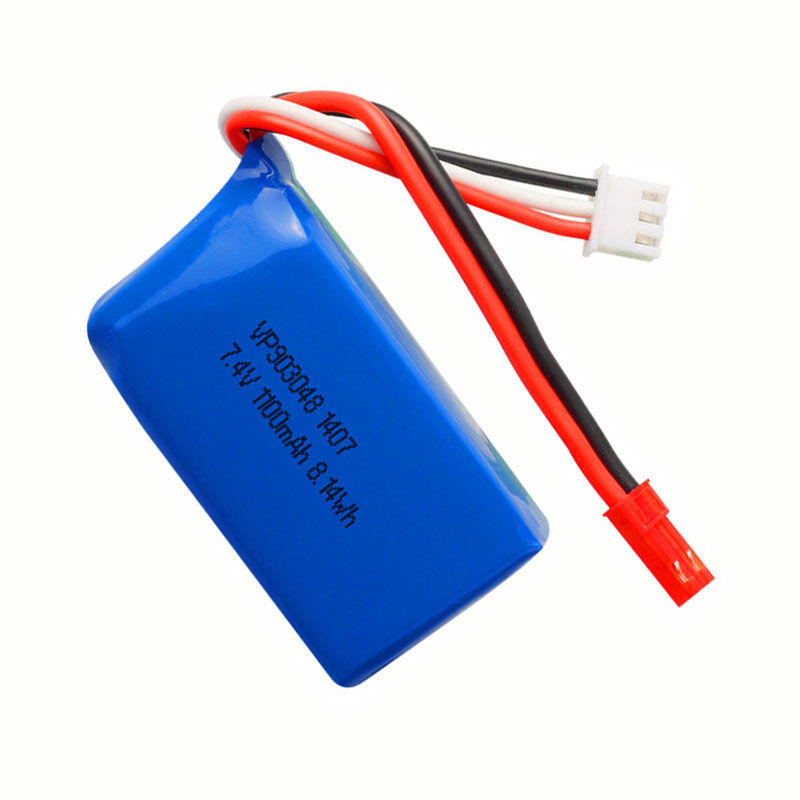
\includegraphics[width=0.6\textwidth]{figuras/imagembateria.png}
    \captionsetup{font=footnotesize}
    \caption{Imagem ilustrativa da bateria selecionada.}
\end{figure}

\end{apendicesenv}